% Fig. 1 (overview). PAGE width (7.1 in = 18.03 cm). Compile: pdflatex overview.tex
% Colours follow paper/scripts/figures/style.py: source and start = GRAY, target labels and student = SLOT[0],
% teacher and weak labels = SLOT[6], text = INK / INK2.
\documentclass[tikz,border=1pt]{standalone}
\usepackage[T1]{fontenc}
\usepackage[scaled]{helvet}
\renewcommand{\familydefault}{\sfdefault}
\usepackage{amsmath}
\usepackage{sfmath}
\usepackage[none]{hyphenat}
\usetikzlibrary{arrows.meta,positioning,calc,shapes.geometric,decorations.pathreplacing,decorations.pathmorphing}
\definecolor{src}{HTML}{8A8985}
\definecolor{tgt}{HTML}{2A78D6}
\definecolor{tea}{HTML}{6250D6}
\definecolor{ink}{HTML}{0B0B0B}
\definecolor{ink2}{HTML}{52514E}
\tikzset{
  >={Stealth[length=4pt,width=3.4pt]},
  every node/.style={font=\scriptsize, text=ink},
  title/.style={font=\footnotesize\bfseries, anchor=north west, inner sep=0pt},
  sub/.style={font=\scriptsize, text=ink2, anchor=north west, inner sep=0pt},
  box/.style={draw, rounded corners=2pt, line width=0.6pt, align=center, inner sep=3pt},
  chip/.style={draw=ink2, line width=0.4pt, fill=white, font=\scriptsize\bfseries, minimum width=9.5pt, minimum height=9.5pt, inner sep=0pt, rounded corners=1pt},
  flow/.style={->, line width=0.8pt, draw=ink2},
  db/.style={cylinder, shape border rotate=90, aspect=0.25, draw=src, fill=src!18, line width=0.5pt, minimum width=0.95cm, minimum height=0.62cm},
  lab/.style={fill=tgt, draw=white, line width=0.3pt},
}
\begin{document}
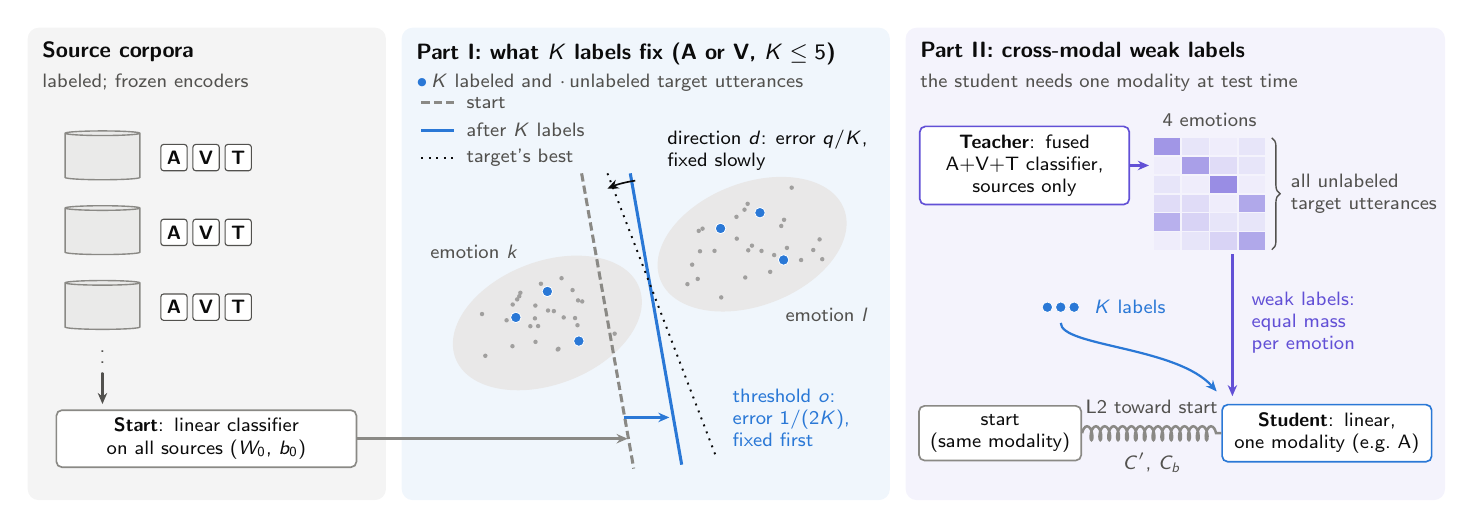
\begin{tikzpicture}
% ------------------------------------------------------------------ panel backgrounds
\fill[src!9, rounded corners=4pt] (0,0) rectangle (4.55,6.0);
\fill[tgt!7, rounded corners=4pt] (4.75,0) rectangle (10.95,6.0);
\fill[tea!7, rounded corners=4pt] (11.15,0) rectangle (18.0,6.0);

% ------------------------------------------------------------------ left: sources and the start
\node[title] at (0.18,5.82) {Source corpora};
\node[sub]   at (0.18,5.42) {labeled; frozen encoders};
\foreach \y/\n in {4.35/1, 3.40/2, 2.45/3} {
  \node[db] (d\n) at (0.95,\y) {};
  \node[chip, right=0.25cm of d\n] (a\n) {A};
  \node[chip, right=0.06cm of a\n] (v\n) {V};
  \node[chip, right=0.06cm of v\n] (t\n) {T};
}
\node[text=ink2] at (0.95,1.85) {$\vdots$};
\node[box, draw=src, fill=white, text width=3.6cm] (start) at (2.27,0.78)
  {\textbf{Start}: linear classifier\\on all sources ($W_0$, $b_0$)};
\draw[flow] (0.95,1.62) -- (0.95,1.22);

% ------------------------------------------------------------------ middle: Part I
\node[title] at (4.93,5.82) {Part I: what $K$ labels fix (A or V, $K\le5$)};
\node[sub]   at (4.93,5.42) {\textcolor{tgt}{$\bullet$}\,$K$ labeled and \textcolor{ink2}{$\cdot$}\,unlabeled target utterances};
\begin{scope}[shift={(5.05,0.2)}]
  % two emotion clouds; centres (1.55,2.05) and (4.15,3.05), midpoint (2.85,2.55)
  \fill[ink2!13] (1.55,2.05) ellipse [x radius=1.25cm, y radius=0.78cm, rotate=21];
  \fill[ink2!13] (4.15,3.05) ellipse [x radius=1.25cm, y radius=0.78cm, rotate=21];
  \node[text=ink2] at (0.62,2.95) {emotion $k$};
  \node[text=ink2] at (5.1,2.15) {emotion $l$};
  \pgfmathsetseed{7}
  \foreach \i in {1,...,26} {
    \pgfmathsetmacro{\u}{rand*1.0}\pgfmathsetmacro{\v}{rand*0.5}
    \fill[ink2!55] ($(1.55,2.05)+(21:\u)+(111:\v)$) circle (0.8pt);
    \pgfmathsetmacro{\u}{rand*1.0}\pgfmathsetmacro{\v}{rand*0.5}
    \fill[ink2!55] ($(4.15,3.05)+(21:\u)+(111:\v)$) circle (0.8pt);
  }
  \foreach \p in {(1.15,2.12),(1.95,1.82),(1.55,2.45)} \fill[lab] \p circle (1.9pt);
  \foreach \p in {(3.75,3.25),(4.55,2.85),(4.25,3.45)} \fill[lab] \p circle (1.9pt);
  % start: direction 100 deg, through (2.25,2.45); after K labels: same direction through the midpoint;
  % target's best: direction 111 deg through the midpoint
  \draw[src, line width=1.1pt, dash pattern=on 3pt off 1.5pt] (1.985,3.95) -- (2.647,0.20);
  \draw[tgt, line width=1.1pt] (2.603,3.95) -- (3.256,0.25);
  \draw[ink, line width=0.7pt, dotted] (2.313,3.95) -- (3.693,0.35);
  % threshold: parallel shift
  \draw[->, tgt, line width=0.8pt] (2.52,0.85) -- (3.10,0.85);
  \node[anchor=west, text=tgt, align=left] at (3.78,0.85) {threshold $o$:\\error $1/(2K)$,\\fixed first};
  % direction: rotation toward the best
  \draw[->, ink, line width=0.6pt] (2.85,2.55) ++(98:1.32) arc[start angle=98, end angle=114, radius=1.32cm];
  \node[anchor=west, align=left] at (2.95,4.25) {direction $d$: error $q/K$,\\fixed slowly};
  % line key
  \draw[src, line width=1.1pt, dash pattern=on 3pt off 1.5pt] (-0.05,4.85) -- ++(0.42,0);
  \node[anchor=west, text=ink2] at (0.40,4.85) {start};
  \draw[tgt, line width=1.1pt] (-0.05,4.50) -- ++(0.42,0);
  \node[anchor=west, text=ink2] at (0.40,4.50) {after $K$ labels};
  \draw[ink, line width=0.7pt, dotted] (-0.05,4.15) -- ++(0.42,0);
  \node[anchor=west, text=ink2] at (0.40,4.15) {target's best};
\end{scope}

% ------------------------------------------------------------------ right: Part II
\node[title] at (11.33,5.82) {Part II: cross-modal weak labels};
\node[sub]   at (11.33,5.42) {the student needs one modality at test time};
\node[box, draw=tea, fill=white, text width=2.45cm] (teach) at (12.66,4.25)
  {\textbf{Teacher}: fused\\A+V+T classifier,\\sources only};
% weak-label matrix: rows = unlabeled target utterances, columns = emotions
\begin{scope}[shift={(14.3,4.38)}]
  \foreach \r/\a/\b/\c/\d in {0/60/15/10/15, 1/10/55/20/15, 2/15/10/65/10, 3/20/20/10/50, 4/45/25/15/15, 5/10/15/25/50} {
    \fill[tea!\a] (0.00,-\r*0.24) rectangle ++(0.34,0.22);
    \fill[tea!\b] (0.36,-\r*0.24) rectangle ++(0.34,0.22);
    \fill[tea!\c] (0.72,-\r*0.24) rectangle ++(0.34,0.22);
    \fill[tea!\d] (1.08,-\r*0.24) rectangle ++(0.34,0.22);
  }
  \node[anchor=south, text=ink2] at (0.71,0.24) {4 emotions};
  \draw[decorate, decoration={brace, amplitude=3pt}, ink2, line width=0.5pt] (1.50,0.22) -- (1.50,-1.20);
  \node[anchor=west, text=ink2, align=left] at (1.62,-0.49) {all unlabeled\\target utterances};
\end{scope}
\draw[flow, draw=tea] (teach.east) -- (14.24,4.25);
% student and the anchor to the start
\node[box, draw=tgt, fill=white, text width=2.45cm] (stud) at (16.5,0.85)
  {\textbf{Student}: linear,\\one modality (e.g.\ A)};
\draw[flow, draw=tea] (15.3,3.12) -- (15.3,1.32);
\node[anchor=west, text=tea, align=left] at (15.42,2.25) {weak labels:\\equal mass\\per emotion};
\node[box, draw=src, fill=white, text width=1.85cm] (st2) at (12.35,0.85) {start\\(same modality)};
\draw[line width=0.9pt, draw=src, decorate, decoration={coil, aspect=0.4, segment length=3.2pt, amplitude=2.5pt}]
  (st2.east) -- (stud.west);
\node[anchor=south, text=ink2] at ($(st2.east)!0.5!(stud.west)+(0,0.13)$) {L2 toward start};
\node[anchor=north, text=ink2] at ($(st2.east)!0.5!(stud.west)+(0,-0.13)$) {$C'$, $C_b$};
\foreach \x in {0,1,2} \fill[lab] ($(12.95,2.45)+(\x*0.17,0)$) circle (1.9pt);
\node[anchor=west, text=tgt] at (13.42,2.45) {$K$ labels};
\draw[flow, draw=tgt] (13.12,2.25) .. controls (13.12,1.95) and (14.6,1.95) .. (15.1,1.38);

% ------------------------------------------------------------------ the start enters the target
\draw[flow, draw=src, line width=1.0pt] (start.east) -- (7.62,0.78);
\end{tikzpicture}
\end{document}
